\documentclass[12pt,notitlepage]{article}
\author{Leo Przybylski \\
\texttt{przybyls@u.arizona.edu}}
\usepackage{graphicx}
\usepackage{listings}
\usepackage{color}
\usepackage{hyperref}
\usepackage{hyperlatex}
\setcounter{htmldepth}{0}

\definecolor{DarkBlue}{rgb}{0,0,0.55}
\definecolor{DarkGreen}{rgb}{0,0.4,0}
\definecolor{Purple}{rgb}{0.5,0,0.5}

\begin{ifhtml}
\newcommand{\sf}[1]{\xml{span style="font-family: sans-serif;"}#1\xml{/span}}
\newcommand{\rm}[1]{\xml{span style="font-family: serif;"}#1\xml{/span}}
\newcommand{\bf}[1]{\xml{span style="font-weight: bold;"}#1\xml{/span}}
\newcommand{\href}[2]{\xml{a href="#1"}#2\xml{/a}}
\newcommand{\HlxStyleSheet}{
  \begin{rawxml}
    <!-- metadata -->
    <meta name="generator" content="S5" />
    <meta name="version" content="S5 1.1" />
    <meta name="presdate" content="\end{rawxml}\HlxDate\begin{rawxml}"/>
    <meta name="author" content="\end{rawxml}\HlxAuthor\begin{rawxml}"/>
    <meta name="company" content="Leosandbox " />
    <!-- configuration parameters -->
    <meta name="defaultView" content="slideshow" />
    <meta name="controlVis" content="hidden" />
    <!-- style sheet links -->
    <link rel="stylesheet" href="ui/kuali/slides.css" type="text/css" media="projection" id="slideProj" />
    <link rel="stylesheet" href="ui/kuali/outline.css" type="text/css" media="screen" id="outlineStyle" />
    <link rel="stylesheet" href="ui/kuali/print.css" type="text/css" media="print" id="slidePrint" />
    <link rel="stylesheet" href="ui/kuali/opera.css" type="text/css" media="projection" id="operaFix" />
    <script src="ui/kuali/slides.js" type="text/javascript"></script>
  \end{rawxml}
}

\newcommand{\maketitle}{
    \xml{div class="slide"}
    \EmptyP{\HlxTitleP}{\HlxBlk\xml{h1}\HlxTitle\xml{/h1}
    \EmptyP{\HlxAuthorP}{\xml{h2}\HlxAuthor\xml{/h2}}{}
    \EmptyP{\HlxDate}{\xml{h3}\HlxDate\xml{/h3}}{}
    \xml{/div}
    }{}}

\end{ifhtml}

\newenvironment{s5presentation}{\endpar%
  \HlxBlk\begin{rawxml}
  <div class="header">
    <div class="header_l">
      <div class="header_r">
      &nbsp;
      </div>
    </div>
  </div>
  <div class="content">
    <div class="content_l">
      <div class="content_r">
        <img src="ui/kuali/blank.gif" id="filler" border="0"/>
<div class="layout">
  <div id="controls"><!-- DO NOT EDIT --></div>
  <div id="currentSlide"><!-- DO NOT EDIT --></div>
  <div id="header">
    <img style="position: relative; top:30px; left: 18px;" src="ui/kuali/logo.png" />
  </div>
  <div id="footer">
    <div class="footer_l">
      <div class="footer_r">
        <h1/>
        <h2>\end{rawxml}\HlxTitle\begin{rawxml}</h2>
      </div>
    </div>
  </div>
</div>
    </div>
  </div>
 </div>
<div class="presentation">
    \end{rawxml}}{\HlxBlk\xml{/div}}
\newenvironment{s5slide}{\xml{div class="slide"}}{\xml{/div}}
\newcommand{\fulltitle}[1]{\title{#1}\htmlonly{\htmltitle{#1}}}

\fulltitle{AccountingDocument Refactoring Using Generics Proposal}


\begin{document}
  \texonly{
    \lstset{language=Java,
      basicstyle=\small,
      keywordstyle=\color{Purple}\bfseries,
      commentstyle=\color{DarkGreen},
      identifierstyle=\color{DarkBlue},
      rangeprefix=\/\/\ ,
      rangesuffix=,
      breaklines=true,
      breakatwhitespace=true,
      includerangemarker=false}
  }
  \maketitle
  \texonly{\tableofcontents \listoffigures} 
  \section{Motivation}
  \verb|AccountingDocument| is currently imposing a class hierarchy restriction of \verb|SourceAccountingLine|
  and \verb|TargetAccountingLine|. This can be problematic for documents that want to share characteristics 
  between Source and Target \verb|AccountingLine| types, but maintain the document hierarchy.
  
  \subsection{Use Cases}
  \subsubsection{LaborExpenseTransferDocument Hierarchy}
  \verb|ExpenseTransferSourceAccountingLine| and \verb|ExpenseTransferTargetAccountingLine| share the same 
  characteristics through the \verb|ExpenseTransferAccountingLineBase| class. Unfortunately, this relationship
  prevents \verb|ExpenseTransferSourceAccountingLine| and \verb|ExpenseTransferTargetAccountingLine| from 
  inheriting from \verb|SourceAccountingLine| and \verb|TargetAccountingLine| respectively. As a result, they 
  cannot be used as Source and Target lines for the \verb|AccountingDocument|
  \newpage
  To illustrate using the \verb|LaborExpenseTransferDocument|
  \begin{figure}[!h]
    \caption{View of the AccountingDocument Parallel Hierarchy}
    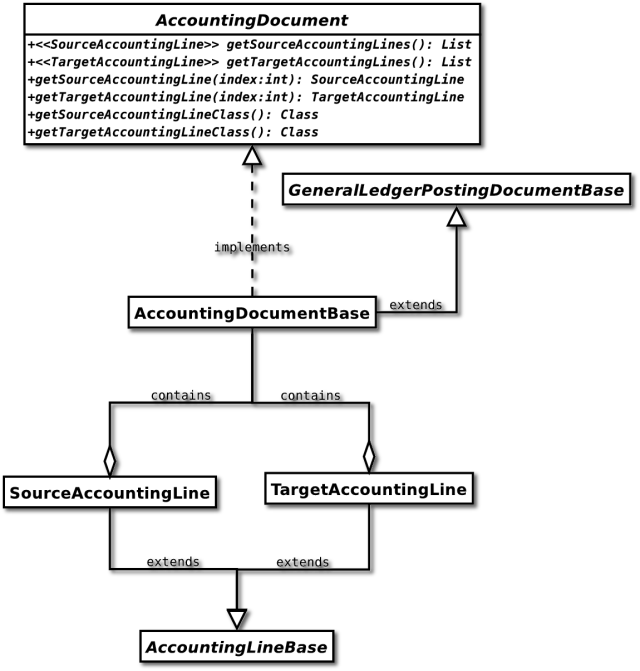
\includegraphics[bb=10 300 300 640]{../Diagrams/AccountingDocumentParallelHierachy_class.png}
  \end{figure}

  The above shows the relationship that requires \verb|AccountingDocument| to use \verb|SourceAccountingLine|
  and \verb|TargetAccountingLine|
  \newpage
  \begin{figure}[!h]
    \caption{View of the ExpenseTransferDocument Hierarchy}
    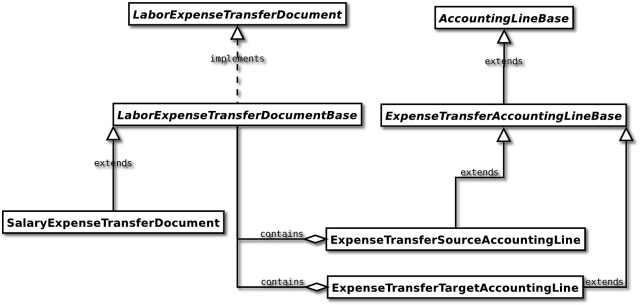
\includegraphics[bb=25 250 400 450]{../Diagrams/ExpenseTransferDocumentHierarchy_class.png}
  \end{figure}
  The diagram above illustrates the \verb|ExpenseTransferDocument| hierarchy

  \begin{figure}[!h]
    \caption{View of the AccountingLine Hierarchy}
    \includegraphics[bb=25 50 450 250]{../Diagrams/AccountingLineHierarchy_class.png}
  \end{figure}
  The diagram above illustrates how \verb|ExpenseTransferSourceAccountingLine| and \verb|ExpenseTransferTargetAccountingLine|
  cannot also be \verb|SourceAccountingLine| and \verb|TargetAccountingLine| respectively due to single inheritance.

  \section{Implementation}
  \subsection{Changes to AccountingDocument and AccountingDocumentBase}
  \subsubsection{AccountingDocument}
  \subsubsection{AccountingDocumentBase}
  \subsection{Changes to KualiAccountingDocumentActionBase}
  \begin{enumerate}
    \item Cast \verb|ActionForm| to \verb|KualiAccountingDocumentFormBase<Source, Target>|. For example, in the \verb|KualiAccountingDocumentActionBase#execute()| method:
      \lstinputlisting[linerange=ExecuteCastStart-ExecuteCastEnd]{../../../../../kuali_project/work/src/org/kuali/kfs/web/struts/action/KualiAccountingDocumentActionBase.java}
      \begin{lstlisting}
        ...
        ...
    }
      \end{lstlisting}
  \end{enumerate}
  \subsection{Changes to KualiAccountingDocumentFormBase}
  \subsection{Changes to Struts Classes}
  EDoc classes that inherit from \verb|AccountingDocument| \verb|AccountingDocumentBase| also require implementations of
  \verb|KualiAccountingDocumentFormBase| and \verb|KualiAccountingDocumentActionBase|. Classes that inherit from require 
  the following refactorings. 
  \begin{enumerate}
    \item Class signature change. For example:
%\verb|public class IndirectCostAdjustmentDocumentActionBase 
%        extends AccountingDocumentBase<SourceAccountingLine, TargetAccountingLine> implements Copyable, Correctable, AmountTotaling {

%public class IndirectCostAdjustmentDocumentFormBase 
%        extends AccountingDocumentBase<SourceAccountingLine, TargetAccountingLine> implements Copyable, Correctable, AmountTotaling {|
  \end{enumerate}
  \subsection{Changes to EDoc Classes}
  EDoc classes that inherit from \verb|AccountingDocument| \verb|AccountingDocumentBase| require the following refactorings.
  \begin{enumerate}
    \item Class signature change. For example:
%\verb|public class IndirectCostAdjustmentDocument 
%       extends AccountingDocumentBase<SourceAccountingLine, TargetAccountingLine> implements Copyable, Correctable, AmountTotaling {|
  \end{enumerate}
  \subsection{Changes to IndirectCostAdjustmentDocument}
    \begin{enumerate}
    \item Remove casting on anything since generics takes care of everything
    \end{enumerate}
    
  \subsection{Changes to ProcurementCardDocument}
    \begin{enumerate}
      \item Remove casting on anything since generics takes care of everything
      \item Remove casting in ProcurementCardTransactionDetail since generics takes care of that too.
      \item Change all references to SourceAccountingLine to ProcurementCardSourceAccountingLine
      \item Change all references to TargetAccountingLine to ProcurementCardTargetAccountingLine
   \end{enumerate}

\end{document}